\chapter{Features of Fit with friends} \label{fitwithf}
This is the overview of the functionalities from the high-fidelity prototype. This is the final product from this research project and the application consists of three different sections.

\section{Logging workouts}
The logging workout section shown in \ref{logworks} is the front page of the application. The bottom navigation includes "My workouts" , "log workout" and "Group workouts". Log workout leads to a user form that consists of three steps. 
\begin{figure}[H]
    \flushright
    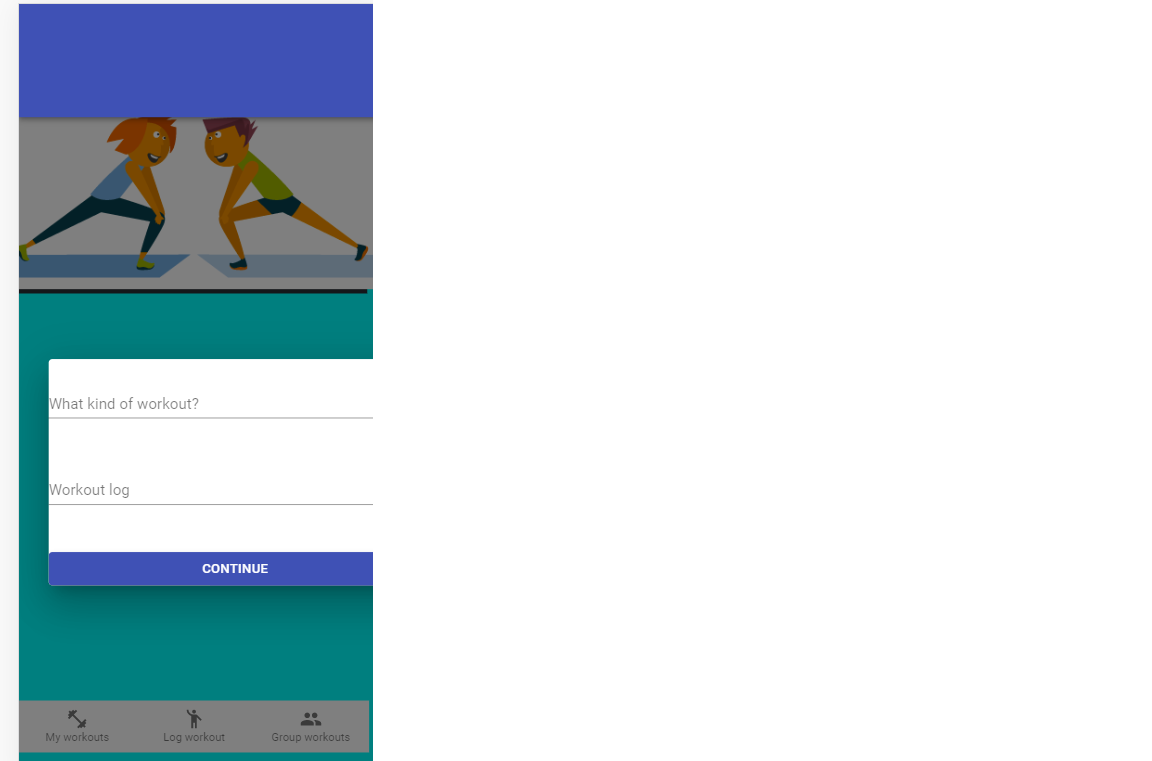
\includegraphics[scale=0.6]{figures/loggingworkouts.png}
    \caption{Logging workouts}
    \label{logworks}
    \end{figure}
In the first step of the form, it asks the user what kind of workout is being logged (gym, running, swimming or other) and the details of the workout. The next step asks the user to confirm the details and it is possible to go back to make changes.

    \begin{figure}[H]
    \flushright
    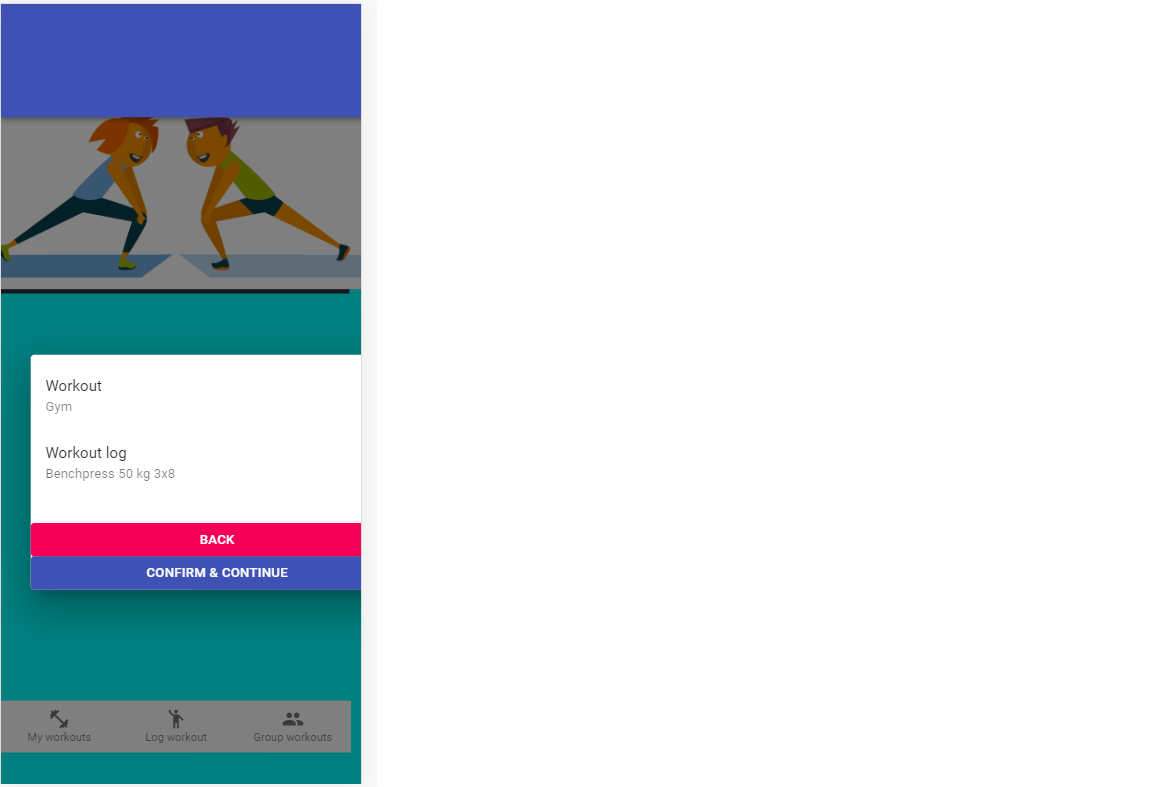
\includegraphics[scale=0.6]{figures/confirmworkouts.png}
    \caption{Confirming input}
\end{figure}


The last step is the success form, the user gets a positive message "Great work" and "Your workout will be added to your log".
\begin{figure}[H]
    \flushright
    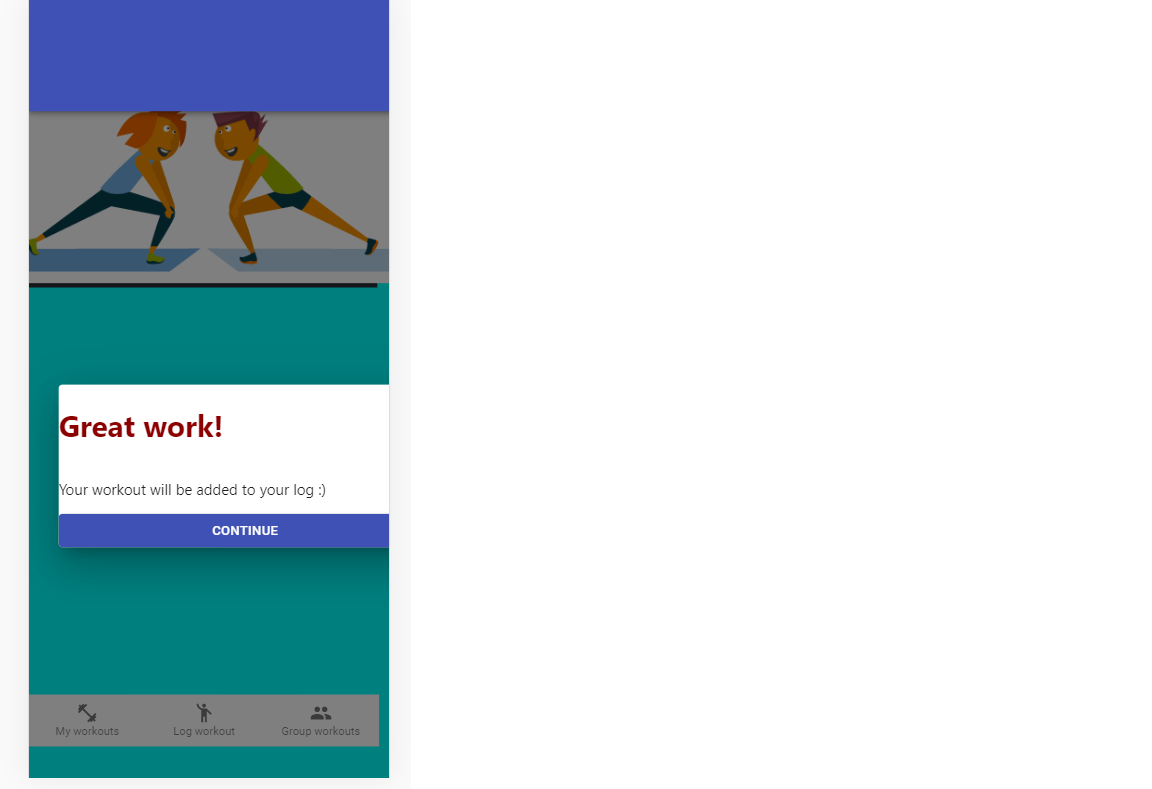
\includegraphics[scale=0.6]{figures/feedbackworkouts.png}
    \caption{Positive feedback}
    \label{positivefeedback}
\end{figure}

\section{My workouts}
My workouts is the personal log of the user. This section consists of all the personal data and information the user has logged in the application. The workout data is presented in tables with the format of exercise, weight, rep scheme. The logged data would show up for the users friends in their social section.
\begin{figure}[H]
    \flushright
    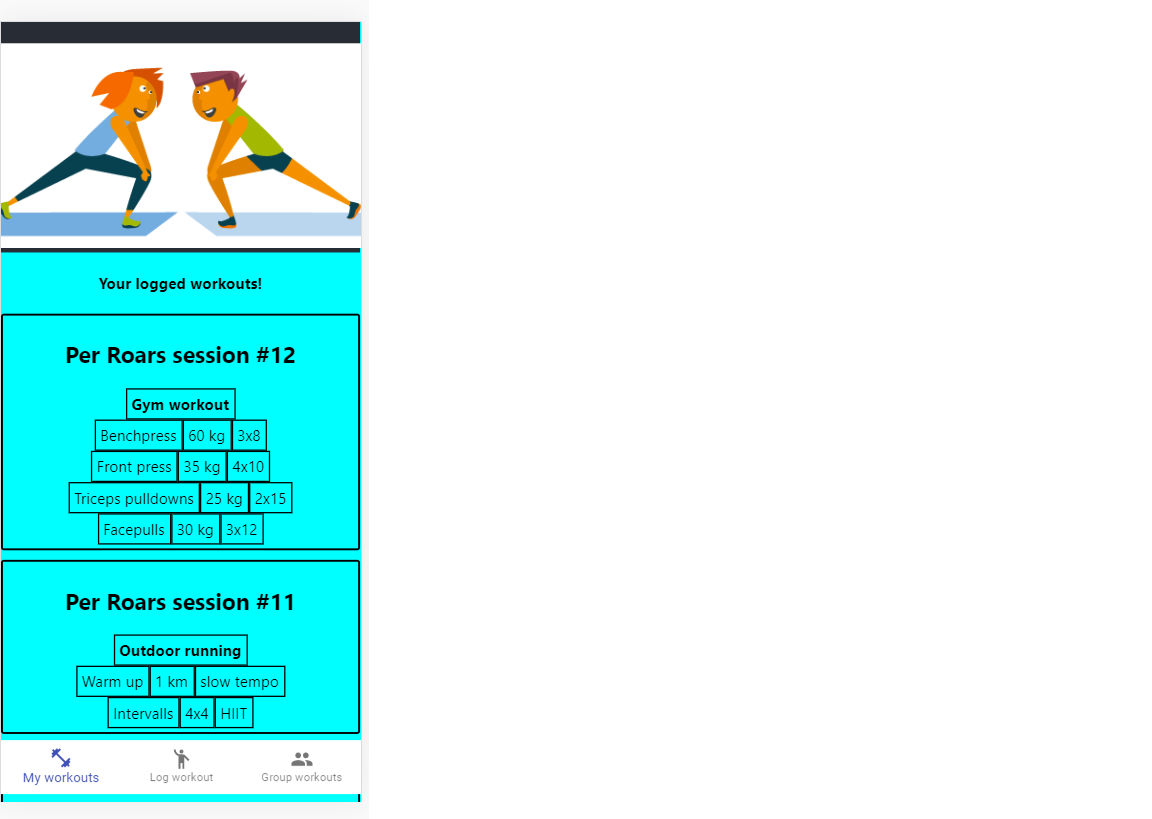
\includegraphics[scale=0.6]{figures/yourloggedworkouts.png}
    \caption{My logged workouts}
    \label{MYLog}
\end{figure}

\section{Social section}
Group workouts is the social section of the application. It includes a personal goal which is supposed to be a long term goal and displays the group goals which are short term goals for the group like going go the gym a total of 10 times a week.
The workout logs of every group member is shown in the social section, this functionality is hidden and if clicked returns a list consisting of all the recent workouts.
\begin{figure}[H]
    \flushright
    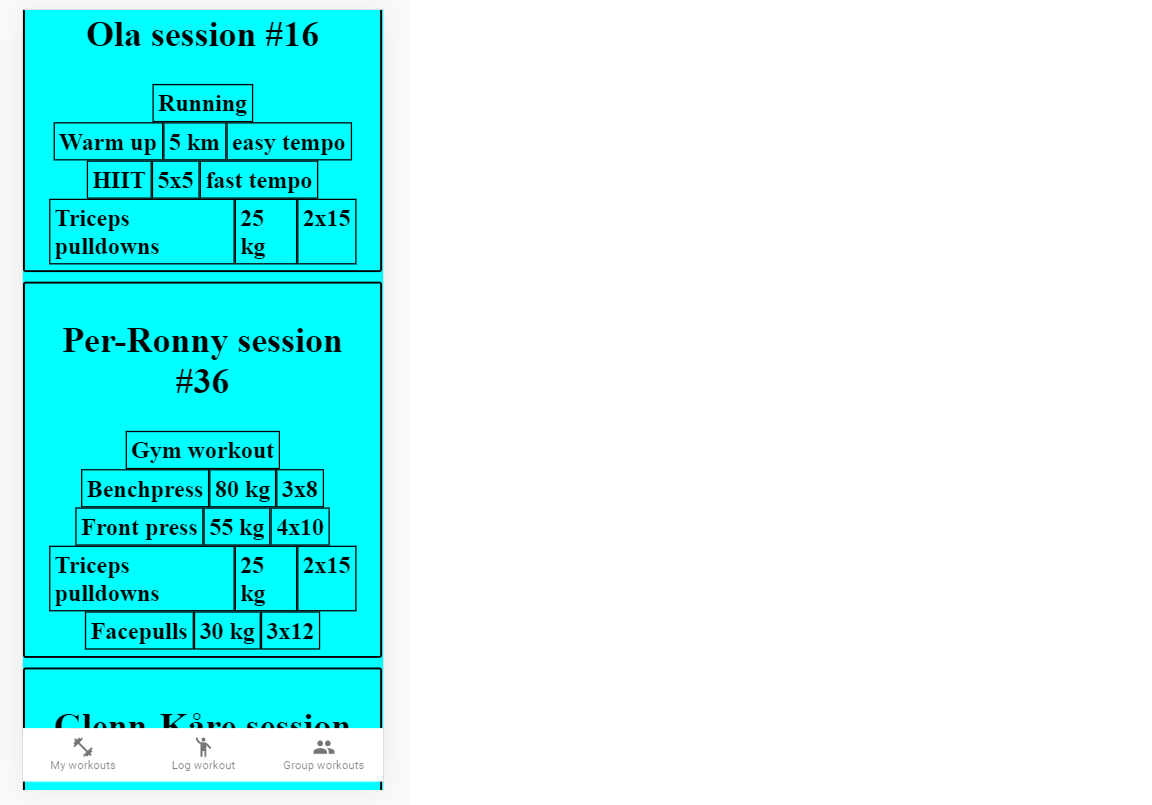
\includegraphics[scale=0.6]{figures/friendsworkoutlogs.png}
    \caption{My friends logged workouts}
    \label{FriendLog}
\end{figure}
This lets the users share information and knowledge about workouts which the users can copy or get inspired and motivated by.
\begin{figure}[H]
    \flushright
    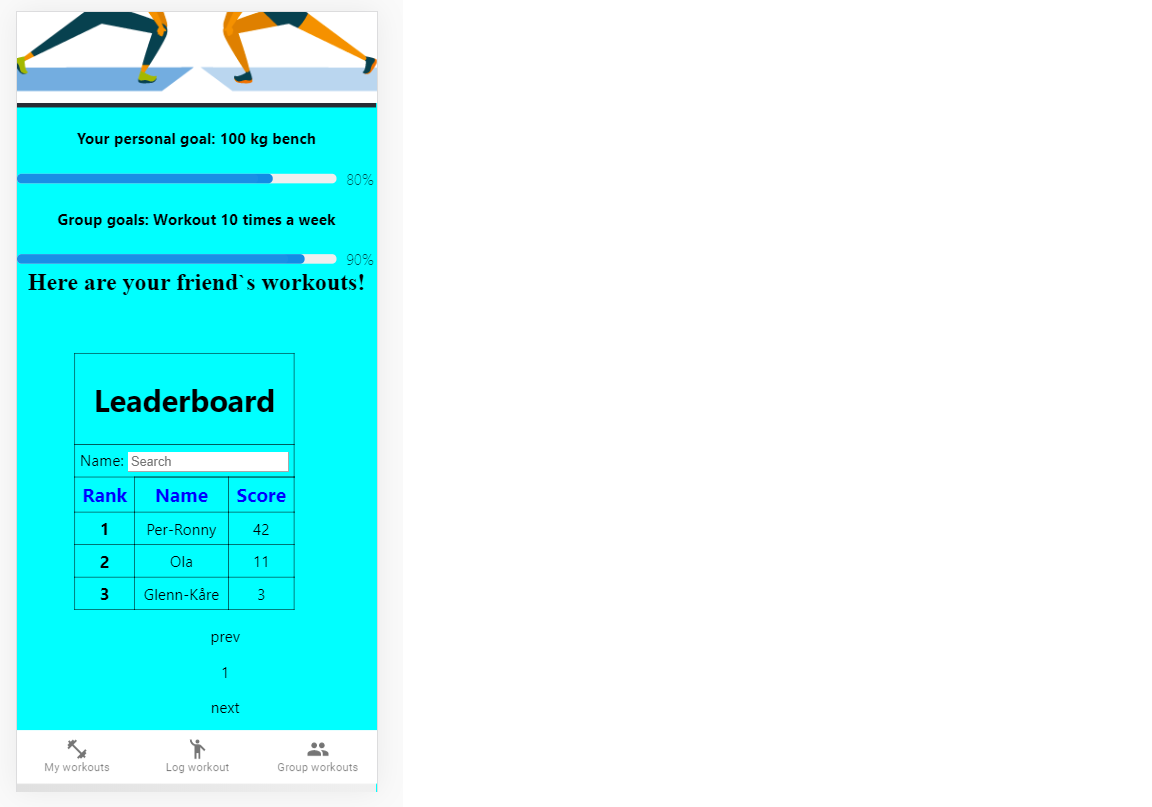
\includegraphics[scale=0.6]{figures/leaderboardandgoals.png}
    \caption{Leaderboard, goals and toggleable friend workouts}
    \label{LeaderB}
\end{figure}
The leaderboard is a gamification design to encourage the group members to compete with each other, a user would get a point if they log a workout and the points form a rank to see who has the most points. The weekly leader would get a notification stating that they have won and then the leaderboard would reset so the users are competing on fair terms every week for their goal.



